\section{Experiments}
\label{sec:experiments}

To validate our method, we performed experiments on two datasets: one is the synthetic half-moons dataset, and the other is the real-world Pascal VOC 2012 dataset.

\subsection{Experiments on the half-moons dataset}
\label{subsec:half-moons}

We use the half-moons dataset provided by Scikit learn \citep{scikit-learn} to generate 10,000 points with a Gaussian noise of $\mathcal{N}(0, x)$, where $x$ ranges between 0.05 and 0.65. The dataset is split into 8,000 training points and 2,000 testing ones. The model used is an MLP.

We evaluate each attribution method using an indicator of performance: the absence of artefacts that do not reflect the model's behaviour. To this end, we use purity, defined as follows.

A well-trained model should classify approximately half of the data points as ``upper moon'' (class 1) and the other half as ``lower moon'' (class 0). Such a model should consider both features of each point important for classification into class 1. Therefore, for a good attribution method, we expect the top 50\% of points—ranked by the quantity $\widetilde{attr}(\textbf{x}; f) = \sum_{i=0}^1 |attr_i(\textbf{x}; f)|$, to be classified as 1, assuming the baseline is chosen as a point to which the network assigns a near-zero score. With this in mind, we define purity as
\begin{equation}
\begin{split}
    \textrm{Purity} &= \frac{1}{N/2}\sum_{\textbf{x}, \, \widetilde{attr}(\textbf{x}; f) \in \textrm{Top 50\% of all attr}} \textrm{argmax}(f(\textbf{x})),
\end{split}
\label{eq:moons-purity}
\end{equation}
where $N$ is the number of data points. We see that this is the average value of the predicted class labels for half of the points. From the above, we infer that, for a well-trained model, we prefer an attribution method that results in the purity close to $1$. In contrast, a random attribution method in this case would result in the purity score of $0.5$. 

In this experiment, we compare the results of attributions from Geodesic IG with methods including Integrated Gradients, GradientShap, InputXGradients \citep{shrikumar2016not}, KernelShap \citep{lundberg2017unified}, Occlusion \citep{zeiler2014visualizing}, and Guided IG \citep{kapishnikov2021guided}.

For all of the methods, we use $(-0.5, -0.5)$ as a baseline. The chosen number of neighbours for the $k$NN part of both Enhanced IG and Geodesic IG is $5$.

\begin{table}[t]
	\centering
	\resizebox{0.3\textwidth}{!}{%
	\begin{tabular}{lccc}
		\toprule
		\textbf{Method} & AUC-Purity $\uparrow$  \\
		\midrule
		Input X Gradients   & 0.328 &  \\
		GradientShap        & 0.483  & \\
		IG                  &0.487 &   \\
		Random                & 0.299 &   \\
		Kernel Shap         & 0.480 &   \\
		Occlusion           & 0.520 &   \\
		Guided IG          & 0.361 & \\
		Enhanced IG       &470& \\
		\midrule
		Geodesic IG  ($k$NN)       & \textbf{0.531}  & \\
		Geodesic IG  (SVI)       & 0.504    &\\
		\bottomrule
	\end{tabular}%
	}
	\caption{Evaluation of different attribution methods on a half-moons dataset with Gaussian noises with standard deviation ranging from 0.05 to 0.65. While our $k$NN-based method outperforms all other methods, we see that unlike larger examples, such as the one summarised in Table \ref{tab:results_voc}, our SVI example struggles to compete due to complexity of tuning hyperparameters.}
	\label{tab:results_moons_2}
\end{table}

We have run our experiment with 5 different seeds and ploted the mean and standard error of the results for different noise levels in Fig. \ref{fig:purity}. We have summarised these results by reporting their area under the curve (AUC) in Table \ref{tab:results_moons_2}. We see that our $k$NN-based Geodesic IG outperforms all other methods, with the gap increaseing with noise. While Occlusion comes close second, we see in Table \ref{tab:results_voc} that the method does not perform well in larger examples with more complex embeddings. To provide better understanding of the comparison of our results with Enhanced IG we present more analysis on this dataset in Section \ref{sec:related_work}.

\begin{figure}[b!]
	\begin{center}
		\centerline{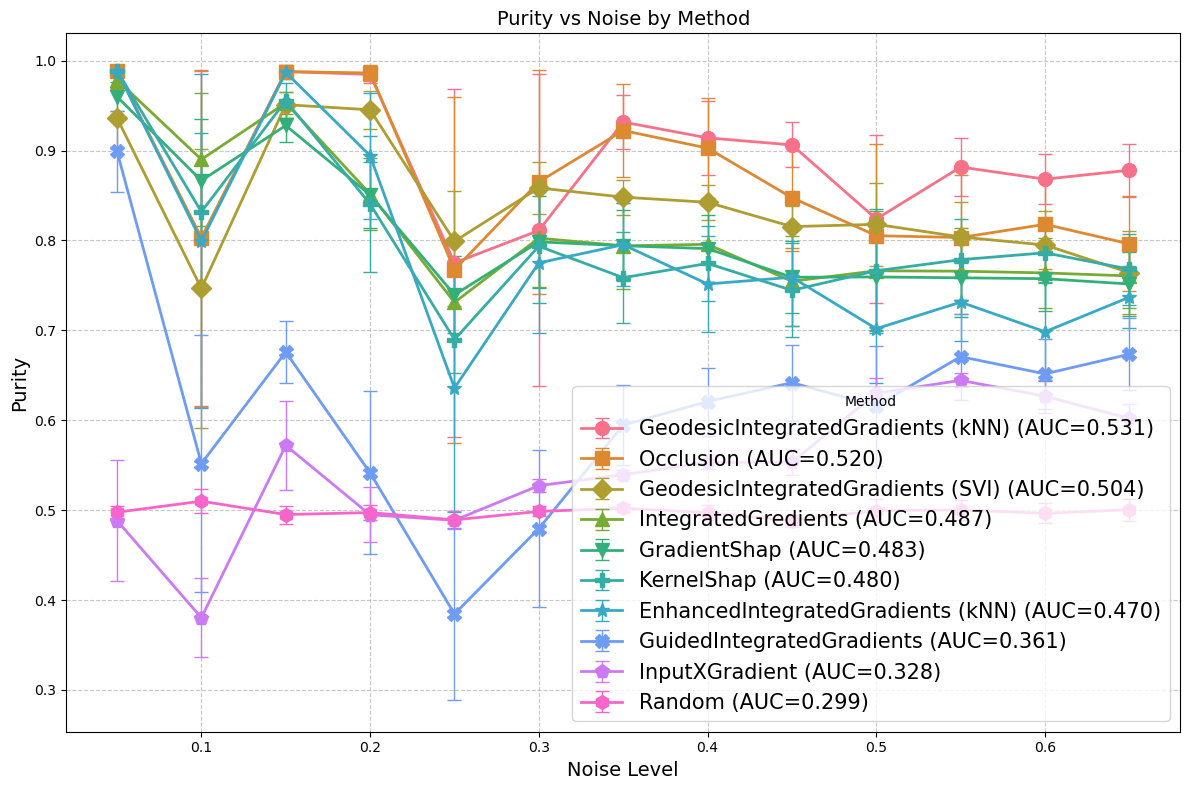
\includegraphics[width=0.95\columnwidth]{figures/purity.png}}
		\caption{A comparison of different attribution methods on half-moons dataset with noise levels ranging from 0.05 to 0.65. Our $k$NN-based method outperforms all, with the gap increase with noise.}
		\label{fig:purity}
	\end{center}
	\vskip -0.3in
\end{figure}


\subsection{Experiments on the Pascal VOC 2012 dataset}
\label{subsec:voc}

To evaluate our method on a real-world dataset, we used the Pascal VOC 2012 dataset \citep{pascal-voc-2012}, which consists of labeled images. We trained a classification head on this dataset and integrated it with the pre-trained ConvNext model \citep{liu2022convnet} from TorchVision to generate predictions for explanation.

For this experiment, we used the same attribution methods as our half-moons experiment, except for the $k$NN-based methods (Enhanced IG and Geodesic IG ($k$NN)) since densely sampling and searching the gradient space of a large model was not practiacal. We applied these attribution methods to classification of 100 randomly selected images. For explainers that require a baseline, such as IG and our proposed method, a uniformly black image was used as the baseline.

To measure the performance of an attribution method, we use 2 different metrics:

\begin{itemize}
    \item \textbf{Comprehensiveness} \citep{deyoung2019eraser}: We maks the top k\% most important features in absolute value, and compute the average change of the predicted class probability compared with the original image. A higher score is better as it indicates masking these features results in a large change of predictions.

    \item \textbf{Log-odds}\footnote{This metric should be called \emph{Log-probabilities}. However, since Log-odds is a commonly used name in the literature, we refer to it as Log-odds.} \citep{shrikumar2017learning}: We mask the top k\% most important features in absolute value, and measure the negative logarithmic probabilities on the predicted class compared with the original one. Lower scores are better.
\end{itemize}

\begin{table}[t]
	\centering
	\resizebox{0.4\textwidth}{!}{%
	\begin{tabular}{lccc}
		\toprule
		\textbf{Method} & AUC-Comp $\uparrow$  & AOC-LO $\uparrow$ \\
		\midrule
        Input X Gradients   & 0.21 & 1.28  \\
        GradientShap        & 0.18  & 1.15  \\
		IG                  &0.21  & 1.25  \\
        Random                & 0.16 & 0.86  \\
        Kernel Shap         & 0.16 & 0.94 \\
        Occlusion           & 0.19 &  1.16 \\
        Guided IG         & 0.20 & 1.18 \\
		\midrule
		Geodesic IG (SVI)         & \textbf{0.27}  & \textbf{1.44}  \\
		\bottomrule
	\end{tabular}%
	}
	\caption{Evaluation of different attribution methods on 100 randomly sampled images from the Pascal VOC test set. Fig. \ref{fig:voc_metrics} shows the curves where these metrics are extracted from.}
	\label{tab:results_voc}
\end{table}

We evaluated these metrics for a range of top-$k\%$, from 1\% to 65\%, as shown in Fig. \ref{fig:voc_metrics}. To summarise performance across different $k\%$ values, we calculated the area under the curve (AUC) for Comprehensiveness. We similarly calculated the area over the curve (AOC) for Log-odds, since the values of this metric are negative. In both cases these are the area between the metric curves and the horizontal line at $y=0$. These results are presented in Table \ref{tab:results_voc}.

Additionally, Fig. \ref{fig:duck} provides a qualitative comparison between Geodesic IG and Integrated Gradients. The results demonstrate that Geodesic IG outperforms other methods in explaining the model's behaviour on the dataset, with a particularly notable improvement in comprehensiveness. Further qualitative comparisons can be found in Appendix \ref{app:voc}.

Using Geodesic IG to explain complex deep learning models comes with several challenges. One major issue is the high computational cost of sampling methods like SVI or HMC. For instance, running the aforementioned experiment on 100 images required 23 hours on an L4 GPU. While computationally expensive, this could be justified in scenarios where accurate explanations are crucial. Another challenge is that the performance of the energy-based geodesic method heavily depends on selecting the right value for $\beta$ in Eq. \ref{eq:energy} and tuning SVI hyperparameters, such as the learning rate. In principle, hyperparameter tuning using metrics like Comprehensiveness or Log-odds could help optimise these parameters. However, due to limited computational resources, we were unable to perform such tuning in this study, though it has the potential to significantly improve results. Lastly, the optimisation nature of these sampling methods can cause the endpoints of the paths to deviate slightly from the baseline and input points, favoring nearby points in lower gradient regions. To address this, we we added a term to the potential energy to correct for these deviations and ensure more accurate alignment with the intended points.  Formally, the extra term is $w \sum_{t \in \text{endpoints}} |\gamma(t) - \gamma_{\text{init}}(t)|_2$, where $w$ is endpoint weight and the first/ last 10\% of the paths are counted as endpoints .